\documentclass[a4paper]{article}
\usepackage[utf8]{inputenc}

%=-=-=-=-=-=-=-=-=-=-=-=-=-=-=-=-=-=-=-=-=-=-=-=-=-=-=-=-=-=-=-=-=-=-=-=-=-=-=-=-
% PREAMBLE
%=-=-=-=-=-=-=-=-=-=-=-=-=-=-=-=-=-=-=-=-=-=-=-=-=-=-=-=-=-=-=-=-=-=-=-=-=-=-=-=-

%%%%%%%%%%%%%%%%%%%%%%%%%%%%%%%%%%%%%%%%%%%%%%%%%%%%%%%%%%%%%%%%%%%%%
% Important styling notes
%%
% For now, to include img.jpg in img/path/to/img.jpg, just use:
% path/to/img.jpg - for details see style.tex
%=-=-=-=-=-=-=-=-=-=-=-=-=-=-=-=-=-=-=-=-=-=-=-=-=-=-=-=-=-=-=-=-=-=-=-=-=-=-=-=-
% Packages
%%
%\usepackage{fullpage} % Package to use full page
\usepackage[top=1in,bottom=1in,left=1in,right=0.7in,heightrounded]{geometry}

\usepackage{parskip}                    % Package to tweak paragraph skipping
\usepackage{amsmath}                    % standard
\usepackage{amssymb}                    % standard - Double R symbol etc.
\usepackage{hyperref}
\usepackage{amsthm}                     % standard - theorem, definition, etc.
\usepackage{multicol}                   % multiple columns for numbering
\usepackage{enumitem}                   % standard - enumerate styles
\usepackage[utf8]{inputenc}
\usepackage{scrextend}                  % indentation
\usepackage{graphicx}                   % standard - add figures
\usepackage{float}                      % standard - figure position, use [H] option
\usepackage{pifont}                     % symbols
\usepackage{gensymb}                    % degree symbol \degree
\usepackage{xcolor}                     % bg color
\hypersetup{
    colorlinks,
    linkcolor={black!50!black},
    citecolor={blue!50!black},
    urlcolor={blue!80!black}
}
\usepackage{framed}                     % bg color
\usepackage[T1]{fontenc}                % small caps
\usepackage{sectsty}                    % headings colour
\usepackage{mathtools}                  % Loads amsmath
\usepackage{amsthm,thmtools,xcolor}     % coloured theorem
\usepackage[toc,page]{appendix}         % reference to appendix
%\usepackage{titlesec}                   % change chapter, section, etc. formats
\usepackage{xifthen}                    % if, else
\usepackage{etoolbox}
% format numbering in theorem, lemma, etc. environment
\AtBeginEnvironment{theorem}{\setlist[enumerate, 1]{font=\upshape,  wide=0.5em, before=\leavevmode}}
\AtBeginEnvironment{lemma}{\setlist[enumerate, 1]{font=\upshape,  wide=0.5em, before=\leavevmode}}
\usepackage[letterspace=150]{microtype} % \textls{<letterspaced text>} % 0 <= letterspace <= 1000, 1000 = M space
\usepackage{letltxmacro}                % renew commands?
\usepackage{minted}                     % package to list code
    % otherwise minted goes off the page
    \setmintedinline{breaklines}
\usepackage{subfig}
\usepackage{eso-pic}                    % title page bg pic
\usepackage{varwidth}
\PassOptionsToPackage{svgnames}{xcolor}
\usepackage{fontawesome}                % \faQuestionCircle
\usepackage{marvosym}                   %\Pointinghand
\usepackage{mdframed}                   % easy outline frames
\usepackage[many]{tcolorbox}            % colour box for theorem styles
\usepackage{array,booktabs,calc} % table figs and text
\usepackage{comment}                    % \begin{comment}
\usepackage{fancyhdr}                   % page headings
\usepackage{mdframed}                   % boxes
\usepackage[backend=biber,sorting=none,style=ieee]{biblatex}
\usepackage{caption}
%%% caption options {
%\DeclareCaptionFont{white}{\color{white}}
\DeclareCaptionFormat{listing}{\colorbox{magenta!30!gray}{\parbox{\textwidth}{#1#2#3}}}
\captionsetup[lstlisting]{format=listing,labelfont={bf,small},textfont=small,skip=-1pt}
%%% }
\addbibresource{bibliography.bib}
\usepackage{url}
\usepackage{textcomp}
\usepackage[makeroom]{cancel}            % crossed symbols
\usepackage{algorithm}
\usepackage[noend]{algpseudocode}
\usepackage{tikz}
\usetikzlibrary{arrows.meta,positioning,quotes} % arrows and nodes in tikz
\usepackage{marginnote}
\usepackage{pgfplots}
\usepackage{pstricks-add,pst-slpe}  % for fancy tikz arrows
%\usepackage{titlesec}                   % title style
\usepackage{lmodern}                    % a font
\usepackage{titletoc} % Required for manipulating the table of contents
\usepackage{titlesec} % Allows customization of titles
\usepackage{fouriernc} % Use the New Century Schoolbook font
\usepackage{booktabs} % things in page margins
\usepackage{stmaryrd } % \varoast
\usepackage{listings} % code listings
\usepackage{longtable} % table across multiple pages
\usepackage{styles/nasm/lang}  % include custom language for NASM assembly.
\usepackage{styles/nasm/style} % include custom style for NASM assembly.



%% extra comments that I don't know where they belong:
% list of ding tags: http://willbenton.com/wb-images/pifont.pdf

%=-=-=-=-=-=-=-=-=-=-=-=-=-=-=-=-=-=-=-=-=-=-=-=-=-=-=-=-=-=-=-=-=-=-=-=-=-=-=-=-
% Colours for various things
%%


\definecolor{shadecolor}{rgb}{1.,0.933,0.96} % bg color, r,g,b <= 1
\definecolor{medium_blue}{RGB}{60,125,190}
\definecolor{dark_blue}{RGB}{25,60,85}
\definecolor{dark_red}{RGB}{77,16,16}
\definecolor{LightPink}{rgb}{0.92.,0.8,0.84} % bg color, r,g,b <= 1
\definecolor{LighterPink}{rgb}{1.,0.94,0.97} % bg color, r,g,b <= 1
\definecolor{LightestPink}{rgb}{1.,0.95,0.99} % bg color, r,g,b <= 1
\definecolor{DarkestPink}{rgb}{0.36, 0.0, 0.18}
\definecolor{DarkerPink}{rgb}{0.41, 0.0, 0.21}
\definecolor{DarkPink}{rgb}{0.55, 0.05, 0.37}
\definecolor{lightestestpink}{RGB}{255,248,252}
\definecolor{codegray}{rgb}{0.5,0.5,0.5}
\definecolor{codegrayblue}{rgb}{0.35,0.35,0.47}



%=-=-=-=-=-=-=-=-=-=-=-=-=-=-=-=-=-=-=-=-=-=-=-=-=-=-=-=-=-=-=-=-=-=-=-=-=-=-=-=-
% Define my own theorem styles
%%

% "base" styles
\declaretheoremstyle[
  headfont=\color{DarkPink}\bfseries,
  bodyfont=\itshape,
]{colored}

\declaretheoremstyle[
  headfont=\color{DarkPink}\bfseries,
  bodyfont=\normalfont,
]{colored_upright}

% theorems (corollaries, etc) themselves, inherit from my style above
% Usage:
% \begin{theorem} \end{theorem}, \begin{lemma} \end{lemma}, ...
\declaretheorem[
	numberwithin=section,
 	style=colored,
	name=\textsc{Theorem},
]{theorem}

\tcolorboxenvironment{theorem}{
  boxrule=0pt,
  boxsep=2pt,
  colback={magenta!25!white},
  colframe=DarkPink,
  enhanced jigsaw, 
  borderline west={2pt}{0pt}{DarkPink},
  sharp corners,
  before skip=5pt,
  after skip=5pt,
  breakable,
  right=0mm % for equations
}

\declaretheorem[
	numberwithin=section,
 	style=colored,
	name=\textsc{Corollary},
]{corollary}

\tcolorboxenvironment{corollary}{
  boxrule=0pt,
  boxsep=1pt,
  colback={magenta!10!white},
  colframe=DarkPink,
  enhanced jigsaw, 
  borderline west={2pt}{0pt}{DarkPink},
  sharp corners,
  before skip=5pt,
  after skip=5pt,
  breakable,
  right=0mm % for equations
}

\declaretheorem[
	numberwithin=section,
	style=colored,
	name=\textsc{Lemma},
]{lemma}

\tcolorboxenvironment{lemma}{
  boxrule=0pt,
  boxsep=1pt,
  colback={magenta!10!white},
  colframe=DarkPink,
  enhanced jigsaw, 
  borderline west={2pt}{0pt}{DarkPink},
  sharp corners,
  before skip=5pt,
  after skip=5pt,
  breakable,
  right=0mm % for equations
}

\declaretheorem[
	numberwithin=section,
	style=colored,
	name=\textsc{Definition},
]{definition}

\tcolorboxenvironment{definition}{
  boxrule=0pt,
  boxsep=1pt,
  colback={magenta!25!white},
  colframe=DarkPink,
  enhanced jigsaw, 
  borderline west={2pt}{0pt}{DarkPink},
  sharp corners,
  before skip=5pt,
  after skip=5pt,
  breakable,
  right=0mm % for equations
}

\declaretheorem[
	numberwithin=section,
  	style=colored,
  	name=\textsc{Example},
]{exmp}

\declaretheorem[
	numberwithin=section,
  	style=colored,
  	name=\textsc{Solution},
]{soln}

%%% code listings
\lstdefinestyle{code1}{
    backgroundcolor=\color{lightestestpink},   
    commentstyle=\color{codegrayblue},
    keywordstyle=\color{DarkerPink},
    numberstyle=\tiny\color{codegray},
    stringstyle=\color{black!40!cyan},
    basicstyle=\small\ttfamily,
    breakatwhitespace=false,
    breaklines=true,        
    captionpos=t,             
    keepspaces=true,        
    numbers=left,           
    numbersep=5pt,
    showspaces=false, 
    showstringspaces=false,
    showtabs=false,
    tabsize=4
}

\lstset{style=code1}

%=-=-=-=-=-=-=-=-=-=-=-=-=-=-=-=-=-=-=-=-=-=-=-=-=-=-=-=-=-=-=-=-=-=-=-=-=-=-=-=-
% Headers (size, font, colour)
%%




\makeatletter
\renewcommand{\@seccntformat}[1]{\llap{\textcolor{DarkestPink}{\csname the#1\endcsname}\hspace{1em}}}                    
\renewcommand{\section}{\@startsection{section}{1}{\z@}
{-4ex \@plus -1ex \@minus -.4ex}
{1ex \@plus.2ex }
{\normalfont\large\sffamily\bfseries\textcolor{DarkestPink}}}
\renewcommand{\subsection}{\@startsection {subsection}{2}{\z@}
{-3ex \@plus -0.1ex \@minus -.4ex}
{0.5ex \@plus.2ex }
{\normalfont\sffamily\bfseries\textcolor{DarkestPink}}}
\renewcommand{\subsubsection}{\@startsection {subsubsection}{3}{\z@}
{-2ex \@plus -0.1ex \@minus -.2ex}
{.2ex \@plus.2ex }
{\normalfont\small\sffamily\bfseries\textcolor{DarkestPink}}}                        


%=-=-=-=-=-=-=-=-=-=-=-=-=-=-=-=-=-=-=-=-=-=-=-=-=-=-=-=-=-=-=-=-=-=-=-=-=-=-=-=-
% Numberings, counters and spacings
%%
\numberwithin{equation}{section} % section number in eq/s
\setlength{\jot}{7pt} % spacing in split, gathered env/s



%% Custom examples
%% Output - Example 1,2,...
\newcounter{example}
\newenvironment{example}[1][]{\refstepcounter{example}\par\medskip
   \textbf{Example~\theexample. #1} \rmfamily}{\medskip}
%%%%%%%%%%%% End of unused %%%%%%%%%%%%



%=-=-=-=-=-=-=-=-=-=-=-=-=-=-=-=-=-=-=-=-=-=-=-=-=-=-=-=-=-=-=-=-=-=-=-=-=-=-=-=-
% Paths
%%
\graphicspath{ {./img/} } % figures' path - can look up files directly from there


%=-=-=-=-=-=-=-=-=-=-=-=-=-=-=-=-=-=-=-=-=-=-=-=-=-=-=-=-=-=-=-=-=-=-=-=-=-=-=-=-
% User defined macros (math mode)
%%


% Curly braces under text. Usage: \myunderbrace{upper}{lower}
\newcommand{\myunderbrace}[2]{\mathrlap{\underbrace{\phantom{#1}}_{#2}} #1}
\newcommand{\setR}{\mathbb{R}} % \ouble R
\newcommand{\setRn}{\mathbb{R}^n} %  double R^n
\newcommand{\setN}{\mathbb{N}} % double N
\newcommand{\setZ}{\mathbb{Z}} % double Z
\let\oldemptyset\emptyset
\let\emptyset\varnothing % nice - looking empty set symbol
\newcommand{\fancyN}{\mathcal{N}} % null space
\newcommand{\fancyR}{\mathcal{R}} % range

\newcommand{\bx}{\textbf{x}}
\newcommand{\by}{\textbf{y}}
\newcommand{\bb}{\textbf{b}}
\newcommand{\bA}{\textbf{A}}
\newcommand{\bB}{\textbf{B}}
\newcommand{\bI}{\textbf{I}}
% double bars as in norm
\newcommand{\norm}[1] {\lVert #1 \rVert} 
\newcommand{\trans}[1]{#1^{\top}}

\newcommand{\mean}[1]{\bar{#1}}
\newcommand{\var}{\sigma^2}

\newcommand{\partdevx}[1]{\frac{\partial #1}{\partial x}}
\newcommand{\partdevxx}[1]{\frac{\partial #1}{\partial x}}
\newcommand{\partdevxn}[1]{\frac{\partial^n #1}{\partial x^n}}
\newcommand{\partdevy}[1]{\frac{\partial #1}{\partial x}}
\newcommand{\partdevyy}[1]{\frac{\partial #1}{\partial y}}
\newcommand{\partdevyn}[1]{\frac{\partial^n #1}{\partial y^n}}

% text above = symbol
\newcommand{\overeq}[1]{\ensuremath{\stackrel{#1}=}} 
\newcommand{\greatersmaller}{%
  \mathrel{\ooalign{\raisebox{.6ex}{$>$}\cr\raisebox{-.6ex}{$<$}}}
} % greater and smaller symbols on top of each other, same line

%=-=-=-=-=-=-=-=-=-=-=-=-=-=-=-=-=-=-=-=-=-=-=-=-=-=-=-=-=-=-=-=-=-=-=-=-=-=-=-=-
% User defined macros (non math)

\newcommand{\qedblack}{$\hfill\blacksquare$} % black square end of line
\newcommand{\qedwhite}{\hfill \ensuremath{\Box}} % white square end of line
\newcommand{\hquad}{\hskip0.5em\relax}% half quad space
%\newcommand{\TODO}{\textcolor{red}{\bf TODO!}\;}

\newcommand{\TODO}[1][]{%
    \ifthenelse{\equal{#1}{}}{\textcolor{red}{\bf TODO!}\;}{\textcolor{red}{\textbf {TODO:} #1}\; }%
}
\newcommand{\B}[1]{\textbf{\textup{#1}}} % bold and upright
\renewcommand{\labelitemi}{\scriptsize$\textcolor{DarkPink}{\blacksquare}$} % itemize - squares instead of bullets
\newcommand{\emphasis}[1]{\textls{#1}}

\LetLtxMacro{\originaleqref}{\eqref}
\renewcommand{\eqref}{Eq.~\originaleqref}
\renewcommand*{\eqref}[1]{Eq.~\originaleqref{#1}}





% background images
%%%%%%%
\newcommand\BackgroundPic{%
\put(0,0){%
\parbox[b][\paperheight]{\paperwidth}{%
\vfill
%\centering

\includegraphics[width=0.125\paperwidth,height=\paperheight,%
]{img/background_02.png}% use ,keepaspectratio
\vfill
}}}
%%%%%%%
% end of background image
%%%%%%%%%%%%%% my own frame
\newmdenv[topline=false,bottomline=false]{leftrightbox}
%%%%%%%%%%%%% end
%%%%%%%%%%%%% my own comment
\newcommand{\mycomment}[1]{\begin{leftrightbox}\Pointinghand~\textbf{Comment:}~#1 \end{leftrightbox}}
%%%%%%%%%%%%% end
% my custom note https://tex.stackexchange.com/questions/301993/create-custom-note-environment-with-tcolorbox
\newmdenv[
    topline=false,
    bottomline=false,
    rightline=false,
    innerrightmargin=0pt
]{siderule}
\newenvironment{mynote}%
    {\begin{siderule}\textbf{\Pointinghand~Note:}}
    {\end{siderule}}
%%%%%%%%%%%%% my own box
\newcommand{\boxone}[1]{\begin{tcolorbox}[colback = LighterPink,colframe=LightPink]
#1
\end{tcolorbox}}
%%%%%%%%%%%%% end

\let\oldemptyset\emptyset
\let\emptyset\varnothing
%algorithmic
\algdef{SE}[DOWHILE]{Do}{doWhile}{\algorithmicdo}[1]{\algorithmicwhile\ #1}%






\begin{document}
%=-=-=-=-=-=-=-=-=-=-=-=-=-=-=-=-=-=-=-=-=-=-=-=-=-=-=-=-=-=-=-=-=-=-=-=-=-=-=-=-
% GLOBAL STYLES (DOCUMENT SCOPE)
%=-=-=-=-=-=-=-=-=-=-=-=-=-=-=-=-=-=-=-=-=-=-=-=-=-=-=-=-=-=-=-=-=-=-=-=-=-=-=-=-
% caption: Figure 1 -> <bold> Fig. 1 </bold>
\captionsetup[figure]{labelfont={bf},labelformat={default},labelsep=period,name={Fig.}}


%=-=-=-=-=-=-=-=-=-=-=-=-=-=-=-=-=-=-=-=-=-=-=-=-=-=-=-=-=-=-=-=-=-=-=-=-=-=-=-=-
% TITLE PAGE
%=-=-=-=-=-=-=-=-=-=-=-=-=-=-=-=-=-=-=-=-=-=-=-=-=-=-=-=-=-=-=-=-=-=-=-=-=-=-=-=-
%%%%%%%%%%%%%%%%%%%%%%%%%%%%%%%%%%%%%%%%%
% Formal Book Title Page
% LaTeX Template
% Version 2.0 (23/7/17)
%
% This template was downloaded from:
% http://www.LaTeXTemplates.com
%
% Original author:
% Peter Wilson (herries.press@earthlink.net) with modifications by:
% Vel (vel@latextemplates.com)
%
% License:
% CC BY-NC-SA 3.0 (http://creativecommons.org/licenses/by-nc-sa/3.0/)
% 
% This template can be used in one of two ways:
%
% 1) Content can be added at the end of this file just before the \end{document}
% to use this title page as the starting point for your document.
%
% 2) Alternatively, if you already have a document which you wish to add this
% title page to, copy everything between the \begin{document} and
% \end{document} and paste it where you would like the title page in your
% document. You will then need to insert the packages and document 
% configurations into your document carefully making sure you are not loading
% the same package twice and that there are no clashes.
%
%%%%%%%%%%%%%%%%%%%%%%%%%%%%%%%%%%%%%%%%%

%----------------------------------------------------------------------------------------
%	PACKAGES AND OTHER DOCUMENT CONFIGURATIONS
%----------------------------------------------------------------------------------------



%----------------------------------------------------------------------------------------
%	TITLE PAGE
%----------------------------------------------------------------------------------------



\begin{titlepage} % Suppresses headers and footers on the title page

	\centering % Centre everything on the title page
	
	\scshape % Use small caps for all text on the title page
	
	\vspace*{\baselineskip} % White space at the top of the page
	
	%------------------------------------------------
	%	Title
	%------------------------------------------------
	
	\rule{\textwidth}{1.6pt}\vspace*{-\baselineskip}\vspace*{2pt} % Thick horizontal rule
	\rule{\textwidth}{0.4pt} % Thin horizontal rule
	
	\vspace{0.75\baselineskip} % Whitespace above the title
	
	{\LARGE COMPUTER VISION NOTES\\ \Large OBJECT LOCALISATION AND TRACKING\\} % Title
	
	\vspace{0.75\baselineskip} % Whitespace below the title
	
	\rule{\textwidth}{0.4pt}\vspace*{-\baselineskip}\vspace{3.2pt} % Thin horizontal rule
	\rule{\textwidth}{1.6pt} % Thick horizontal rule
	
	\vspace{2\baselineskip} % Whitespace after the title block
	
	%------------------------------------------------
	%	Subtitle
	%------------------------------------------------
	My personal notes on
	
	\vspace*{3\baselineskip} % Whitespace under the subtitle
	
	Object Localisation Techniques; Colour Matching, Mean Shift Tracking, Optical Flow, Lukas Kanade 
	
	\vspace*{3\baselineskip} % Whitespace under the subtitle
	
	%------------------------------------------------
	%	Editor(s)
	%------------------------------------------------
	
	By
	
	\vspace{0.5\baselineskip} % Whitespace before the editors
	
	{\normalfont \Large \mintinline{latex}{0xLeo} (\url{github.com/0xleo}) \\} % Editor list
	
	\vspace{0.5\baselineskip} % Whitespace below the editor list
	
	%\textit{The University of California \\ Berkeley} % Editor affiliation
	
	\vfill % Whitespace between editor names and publisher logo
	
	%------------------------------------------------
	%	Publisher
	%------------------------------------------------
	
	
	\vspace{0.3\baselineskip} % Whitespace under the publisher logo
	
	\today % Date
	
	{DRAFT X.YY} % Draft version
	{\\Missing: \ldots}

\end{titlepage}

%----------------------------------------------------------------------------------------

%\maketitle



%=-=-=-=-=-=-=-=-=-=-=-=-=-=-=-=-=-=-=-=-=-=-=-=-=-=-=-=-=-=-=-=-=-=-=-=-=-=-=-=-
% MAIN DOCUMENT
%=-=-=-=-=-=-=-=-=-=-=-=-=-=-=-=-=-=-=-=-=-=-=-=-=-=-=-=-=-=-=-=-=-=-=-=-=-=-=-=-
\newpage
\tableofcontents
\newpage

\section{Histogram-Based Methods}

\subsection{Histogram backprojection}

\subsubsection{Intuition - model and search image histogram}
In image processing, we are usually interested in histograms of greyscale images. However, often the colour histogram can be used to identify an image region or object. RGB histograms are practically not good enough for matching as the R, G, B components are strongly correlation with the illumination hitting the object. In practice, objects are converted from RGB to HSV (Hue, Saturation, Value) domain. \emphasis{Hue} represents the colour type (blue, yellow, etc.), \emphasis{saturation} represents the vibrancy (how vivid or neutral it is) and \emphasis{value} represents the brightness of the colour. Hence HSV decouples the brightness from the colour description. Therefore when performing colour matching we are only interested in the H and S components, which map to a 2D histogram. More about the HSV domain in \ref{app:hsv_domain}.

\mycomment{
The HS components are often but \textit{not always} a good choice for colour-based detection. They may fail detecting black and white objects since black and white can have any colour (H) and in this case the SV components of the HSV or even the YUV domain are a better choice. However, in this article we stick to HS.
}

\emphasis{Histogram backprojection} answers the question ``where in the image are the colours that belong to the object being looked for?''. We do this by defining a \emphasis{model} image (the object we search for -- a. k.a. \emphasis{target}) and the \emphasis{search} (the whole image where we search in), probing the model over search image and calculating their histogram  similarity at each position.

Just to illustrate the idea, assume that we want to match the greyscale (instead of the 2D) histogram of the garlic in Fig. \ref{fig:peppers_and_garlic}. A part of the top garlic has been chosen as the model. The histogram of the model is shown as well as that of two matching candidates. In this case, the histogram of ``match 2'' is more similar to the model's than one ``match 1'' so we want somehow to register that similarity. The question attempted to be answered in the next section is ``how do we measure the similarity of the histogram of the matching candidate to that of the model?''.
\begin{figure}[H]
    \centering
    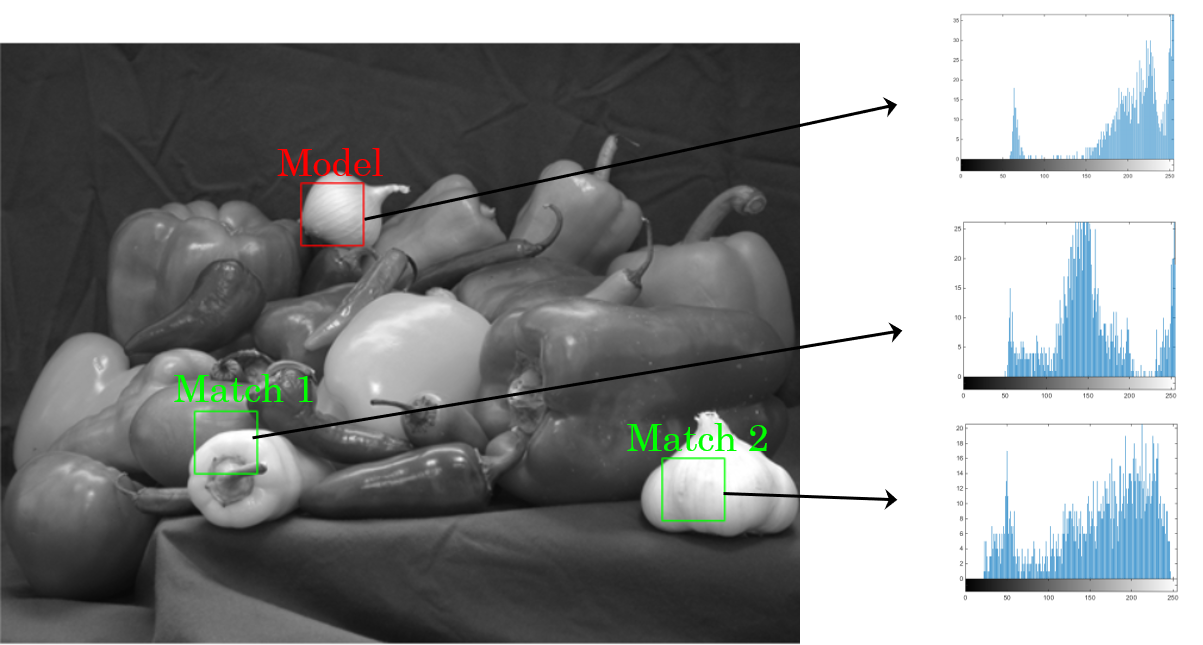
\includegraphics[height=6.5cm]{img/image_hist_different_regions.png}
    \caption{Model and two matches' greyscale histograms.}
    \label{fig:peppers_and_garlic}
\end{figure}


\subsubsection{(optional) The rationale behind defining the ratio histogram}

We assume that 
\begin{enumerate}
    \item the model's histogram (the object we search for) is narrow and tall
    \item and the scene's (whole input image) histogram is rather wide.
\end{enumerate}
It has then been proven (it won't be discussed in this article how as the how is out of scope) that a good histogram similarity measure between the model $M$ and a patch of the image we search it in $I$ is the ratio histogram $R$. $M$ and $I$ need to be pre-calculated and can be divided element-wise, since they have the same range and bins to obtain $R$. The \emphasis{ratio histogram} is a therefore function $R:\mathbb{Z}^2 \rightarrow \mathbb{R}$ that maps a colour $(h,s)$ to some value. If $M(h,s) > I(h,s) \Rightarrow R(h,s) > 1$ that means the model has more pixels of colour $(h,s)$ relative to its total number of pixels compared to $I(h,s)$, and vice versa. If $R(h,s) = 1$, then that means  that the input and model images contain $(h,s)$ at the same degree.

However, because of assumptions (1), (2), $M(h,s) > I(h,s)$ can happen quite often and so long as $M(h,s) > I(h,s) \Rightarrow R(h,s)>1$, e.g. $R(h,s) = 2,3,10$, the exact value does not give much useful information. To summarise, $R$ de-emphasises pixels with colours that do not belong to the model and emphasises the rest.


\subsubsection{A colour matching heuristic}

From the previous section, the conclusion is that it is desirable to clip the ratio histogram to 1, as defined by Swain et al. 
\begin{definition}
For each bin $j$, the ratio histogram is defined as
\begin{equation}
    R_j = \min\left(\frac{M_j}{I_j},1\right)
\end{equation}
, where $M$, $I$ are the model's and input's histograms respectively.
\end{definition}
Note that $j$ does not necessarily have to be a pair $(h,s)$, but it if a histogram bin (index) is quantised it can be a rectangle in the 2D space, such as $[20, 39] \times [50, 69]$. As mentioned before, $R$ associates a colour with its probability of appearing in the model and the next step is the associate each pixel with that probability.

Each pixel of the original image at $(x,y)$ maps to a 2D HS value, by a colour function $c: \mathbb{Z}^2 \leftarrow \mathbb{Z}^2$, by taking $c(x,y)$. Sometimes need an intermediate function $h:\mathbb{Z}^2 \rightarrow \mathbb{Z}^2$ that takes the output of $c$ and quantises it (groups multiple colours in one bin), before it is fed to $R$. For example, $h$ could convert $[0,1,\ldots,179] \times [0,1,\ldots,255]$ to $[0, 19, 39, \ldots,179] \times [0, 24, 49, \ldots, 255]$. The output of $h$ is bed to $R$, which divides $M_j$ to $I_j$ at each bin $j$.To summarise this paragraph we have  defined the following functions in backpropagation:
\begin{itemize}
    \item $c: \mathbb{Z}^2 \rightarrow \mathbb{Z}^2$: maps a pixel at $(x,y)$ to an HS value $(h_j,s_j)$.
    \item $h: \mathbb{Z}^2 \rightarrow \mathbb{Z}^2$ maps a set of values $(h_i,s_i,h_{i+1},s_{i+1},\ldots,h_n,s_n)$ to another $(h,s)$ value by having quantised the range of $h$ and $s$.
    \item $R: \mathbb{Z}^2 \rightarrow [0,1]$ maps an $(h,s)$ value to a probablity.
\end{itemize}
We therefore want to create a new image $b$ where each pixel $(x,y)$ gets assigned its output of $R$ - the measure of how much its colour appears in the model image. 
\begin{equation}
    b(x,y) := R\left(h\left(c(x,y)\right)\right)=
    \min\left(\frac{M\left(h\left(c(x,y)\right)\right)}{I\left(h\left(c(x,y)\right)\right)},1\right) \; \forall \; x,y
\end{equation}
The final step is to find compact regions where $b$ is high. If the shape of the object (model) to detect is generic, then this can be done by convolving $b$ with binary disk mask $D^r$ of radius $r$. Define:
\begin{equation}
    D_{x,y}^r = \left\{
\begin{array}{ll}
      1 & \sqrt{x^2+y^2} \leq r \\
      0 & \textup{otherwise}\\
\end{array} 
\right. 
\end{equation}
Then the probability image $b$ can be convolved with the mask:
\begin{equation}
    b := D^r \ast b
\end{equation}
The $\arg \max$ function to returns the pixel $(x, y)$ with
the maximum value of its argument, i.e. of the $R$ matrix and the $\ast$ symbol denotes convolution. Then Histogram Backprojection algorithm can be then
written
\begin{algorithm}[H]
\caption{Colour matching by histogram backprojection according to Swain et al}
\label{alg:hist_backproj}
\begin{algorithmic}[1]
\Procedure{Hist-BackProj} {ImM, ImI} \Comment{ImM: model, ImI: search image}
\State $M\leftarrow \textup{histogram}(ImM)$
\State $I\leftarrow \textup{histogram}(ImI)$
\For{each histogram bin $j$} \Comment{a bin is a pair $(h,s)$}
\State $R_j = \min\left(\frac{M_j}{I_j}, 1\right)$ \Comment{Divide element-wise}
\EndFor
\State $m \leftarrow rows(M)$
\State $n \leftarrow cols(M)$
\State $b \leftarrow empty_{m \times n}$
\For{y in 0\ldots m-1}
\For{x in 0\ldots n-1}
\State $b_{x,y} \leftarrow R(h(c(x,y)))$ \Comment{b matrix of colour probability}
\EndFor
\EndFor
\State $D^r\leftarrow$ \textup{binary disk of radius r}
\State $b \leftarrow D^r \ast b$ \Comment{Group (by convolving) high probability pixels together.}
\State $x_{obj},y_{obj} \leftarrow \arg \, \underset{x,y}{\mathop{\max }}\,(b)$
\State \textbf{return}  $x_{obj},y_{obj}$
\EndProcedure
\end{algorithmic}
\end{algorithm}

\subsubsection{Histogram backprojection implementation from scratch}

An implementation of Alg. \ref{alg:hist_backproj} has been written in \ref{app:hist_backproj_src}. However, instead of finding the location of the object by the $\arg \max$ function, it applies Otsu's threshold on the $R$ matrix. This automatically selects a threshold $T$ based on the statistics of the histogram of $R$ for which if $R[x,y] < T$, then the pixel at $(x,y)$ is classified as background, else as foreground. Instructions on how to run the implementation code are in \ref{app:hist_backproj_src} and an output is shown below.
\begin{multicols}{2}
    \begin{figure}[H]
        \centering
        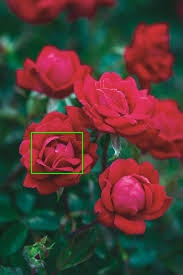
\includegraphics[height=5cm]{img/hist_backproj/rect.jpg}
        \caption{Input image with a ROI of the objects to detect selected.}
        %\label{fig:my_label}
    \end{figure}
    \columnbreak
    \begin{figure}[H]
        \centering
        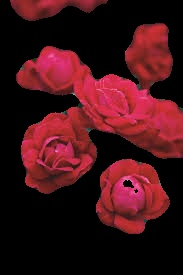
\includegraphics[height=5cm]{img/hist_backproj/res.jpg}
        \caption{Detected objects on the original image.}
        %\label{fig:my_label}
    \end{figure}
\end{multicols}



\subsubsection{Histogram backprojection implementation using OpenCV's API}


OpenCV implements the technique using the \mintinline{python}{cv2.calcBackProject(image, channels, histohram_array, channel_ranges, [scale = 1])} method (in Python). Its invocation looks like:\\
\mintinline{python}{cv2.calcBackProject(search_image, channels, model_histogram, channel_ranges, [scale = 1])}
\begin{itemize}
    \item \mintinline{python}{search_image}: the input image, e.g. in HSV.
    \item \mintinline{python}{channels}: which channels of the original image and the model to select in order to draw its histogram, e.g. \mintinline{python}{channels = [0,1] -> H, S}.
    \item \mintinline{python}{model_histogram}: histogram of the model (ROI), needs to be pre-calculated.
    \item \mintinline{python}{channel_ranges}: set it to \mintinline{python}{[0,180,0,256]} to select the full range of H, S components.
\end{itemize}
The code listing in \ref{app:hist_backproj_src_opencv} works similarly with the one in \ref{app:hist_backproj_src}, expecting two clicks from the user to define a bounding box around a sample of the object to detect. It also performs similarly on the same images, showing some black spots on roughly the same positions.


\subsubsection{Histogram backprojection summary}
\begin{multicols}{2}
    \begin{itemize}
        \item[\textcolor{DarkPink}{\ding{51}}] Fast -- can easily be used in real time.
        \item[\textcolor{DarkPink}{\ding{51}}] Relatively immune to noise and illumination changes.
        \item[\textcolor{DarkPink}{\ding{51}}] Simple to implement.
    \end{itemize}
    
    \columnbreak
    \begin{itemize}
        \item[\textcolor{DarkPink}{\ding{55}}] Not effective against non-compact objects.
        \item[\textcolor{DarkPink}{\ding{55}}] Does not use any knowledge about the shape or position of the detected object -- only its colour.
    \end{itemize}
\end{multicols}





\subsection{Mean Shift Tracking}


\subsubsection{Mean Shift algorithm idea}

% ref https://ieeexplore.ieee.org/document/400568/
Mean shift is a non-parametric feature-space analysis technique for locating the maxima of a density function, a so-called mode-seeking algorithm. In image processing, it's used for tracking.

% ref http://campar.in.tum.de/twiki/pub/Chair/TeachingWs12TDCV/mean_shift.pdf
Given some points $\bx_1, \bx_2, \ldots, \bx_n$ with $d$ dimensions (``features''), for each data point, mean shift defines a window around it
and computes the mean of data point. Then it shifts the centre of window to the mean and repeats the algorithm till the window stops moving. In image processing, feature space is often the colour space. Table \ref{tab:mean_shift_steps} illustrates the iterations until the algorithm converges.

Mean shift is a nonparametric iterative algorithm. It considers each point sampled from a probability distribution, i.e. each point is most likely found at its actual measured position, but it can also be in a neighbourhood around it.

% ref: fig http://campar.in.tum.de/twiki/pub/Chair/TeachingWs12TDCV/mean_shift.pdf

\begin{longtable}{ccc}
\caption{Mean shift update steps shown on a very high level -- in this case the new centre is simply the centroid, until converge (last row).} \label{tab:mean_shift_steps}
\endfirsthead % required
\endhead % required
\toprule
Current centre (blue) & Mean shift vector & New centre (yellow)\\
\midrule
  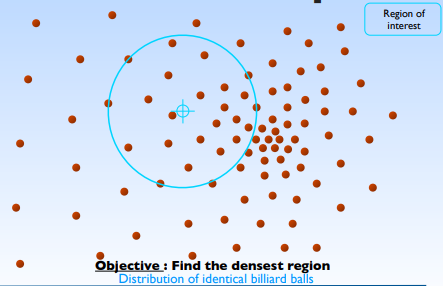
\includegraphics[width=0.32\textwidth] {img/mean_shift/ROI_densest_01.PNG} &
  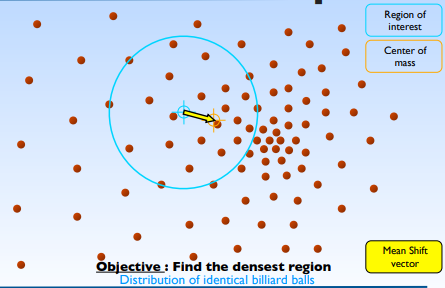
\includegraphics[width=0.32\textwidth] {img/mean_shift/ROI_densest_03.PNG} &
  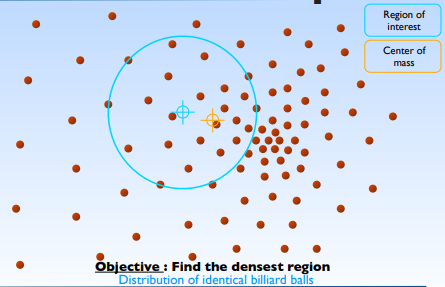
\includegraphics[width=0.32\textwidth] {img/mean_shift/ROI_densest_02.PNG} \\
  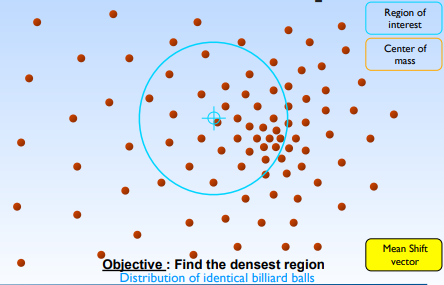
\includegraphics[width=0.32\textwidth] {img/mean_shift/ROI_densest_05.PNG} &
  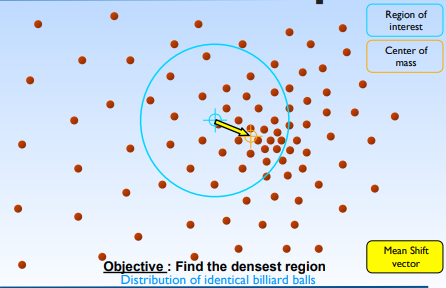
\includegraphics[width=0.32\textwidth] {img/mean_shift/ROI_densest_07.PNG} &   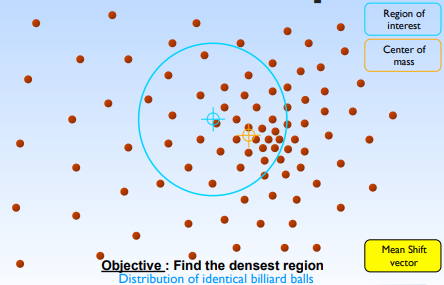
\includegraphics[width=0.32\textwidth] {img/mean_shift/ROI_densest_08.PNG} \\
  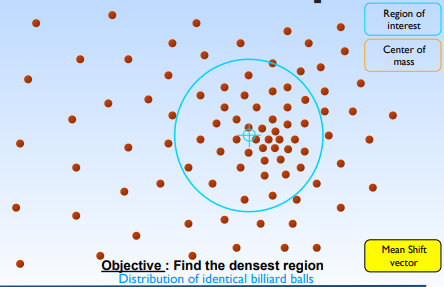
\includegraphics[width=0.32\textwidth] {img/mean_shift/ROI_densest_09.PNG} &
  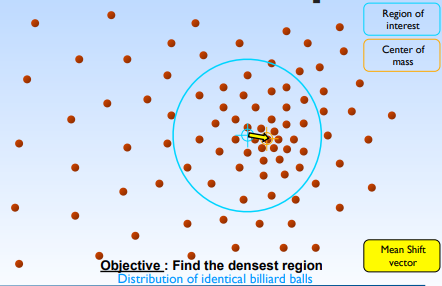
\includegraphics[width=0.32\textwidth] {img/mean_shift/ROI_densest_11.PNG} &
  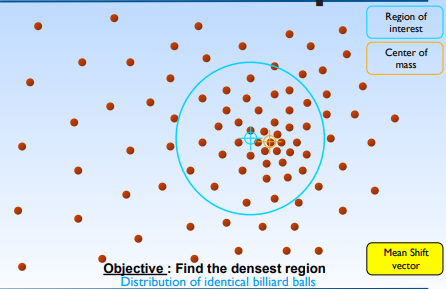
\includegraphics[width=0.32\textwidth] {img/mean_shift/ROI_densest_12.PNG} \\
  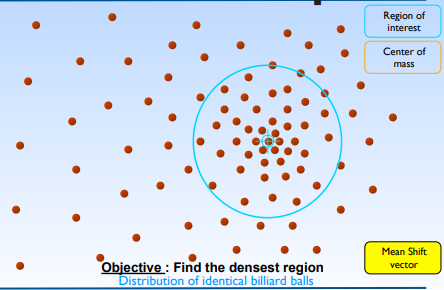
\includegraphics[width=0.32\textwidth] {img/mean_shift/ROI_densest_13.PNG} &
  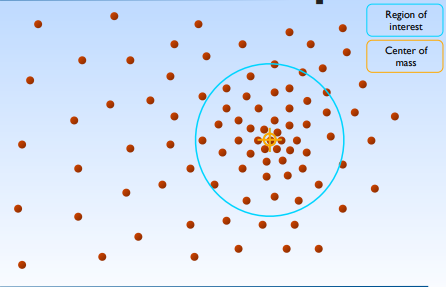
\includegraphics[width=0.32\textwidth] {img/mean_shift/ROI_densest_15.PNG} &
  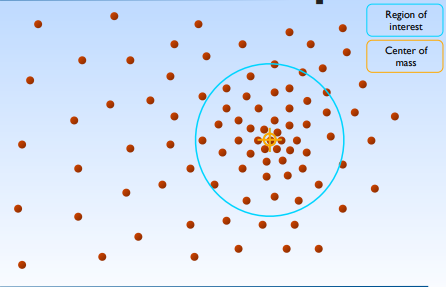
\includegraphics[width=0.32\textwidth] {img/mean_shift/ROI_densest_15.PNG}
\end{longtable}

\faQuestionCircle \; How do we find the peak towards which the circle should move?

\faCheckCircle \; The circle should move towards the densest point of the distribution of all points within the ROI. The peak is found by superimposing all the individual probability distributions around each point and finding the $N$ highest maxima of the result ($N$ is the number of classes we want to have).
% TODO: fig http://robot-develop.org/wp-content/uploads/2012/03/seg3.pdf

\faQuestionCircle \; How do we convert a set of discrete input points to a continuous density function so that we can find the maxima (Fig. \ref{fig:discr_points_to_cont_line})?
\begin{figure}[H]
    % ref http://robot-develop.org/wp-content/uploads/2012/03/seg3.pdf
    \centering
    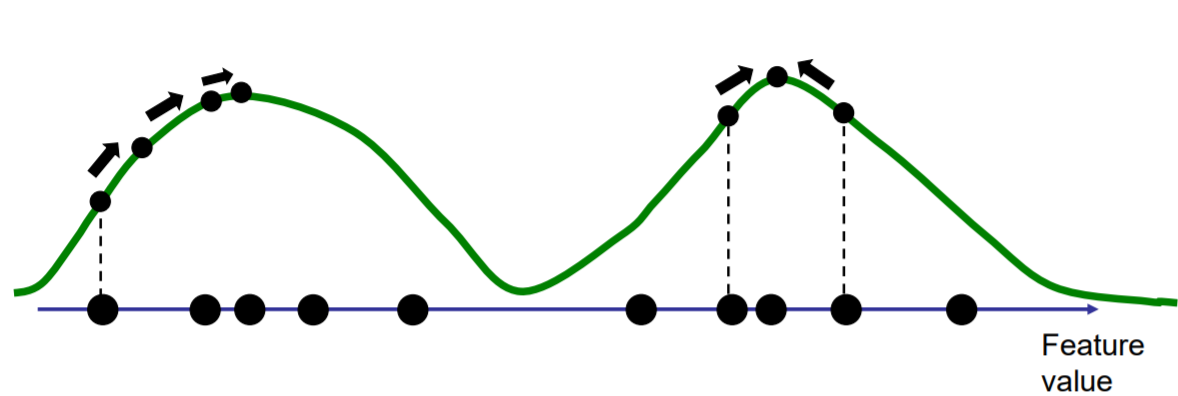
\includegraphics[height=4cm]{img/mean_shift/points_to_cont_green_line.PNG}
    \caption{The green curve is what we roughly want to generate from the 1D input points. The arrows simply show the path gradient ascent would follow to locate the maxima.}
    \label{fig:discr_points_to_cont_line}
\end{figure}
% ref http://robot-develop.org/wp-content/uploads/2012/03/seg3.pdf
\faCheckCircle \; Let us define a kernel function.
\begin{definition}
A \emphasis{kernel} is a real-valued function of the points $\bx_1,\, \bx_2,\, \ldots, \, \bx_n$ that satisfies the following properties:
\begin{enumerate}
    \item $K$ is maximum at $\textbf{0}$, non increasing, and decays away from the maximum.
    \item $K$ is radially symmetric.
    \item $K(\bx) \geq 0$.
    \item $\int_{\setR^d} K(\bx)\, d\bx=1$
\end{enumerate}
\label{def:kernel_func}
\end{definition}

Then for each input point, its kernel function should look roughly as follows.
\begin{figure}[H]
    \centering
    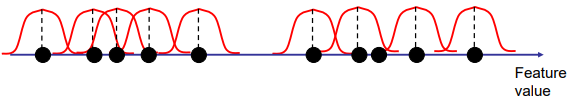
\includegraphics[height=2.0cm]{img/mean_shift/black_points_kernel_functions.PNG}
    \caption{The kernel functions $K(\bx - \bx_i)$, where $\bx_i$ are the input points.}
    \label{fig:my_label}
\end{figure}
If we allocate each point $\bx_i$ its own kernel $K(\bx - \bx_i)$, then by summing all $N$ of them and diving by a constant $C$ to normalise the result we can get a probability density function (PDF):
\begin{equation}
  f(\bx) = \frac{1}{C}\sum \limits _{i=1} ^{N} {K(\bx - \bx_i)}   
\end{equation}
\begin{figure}[H]
    \centering
    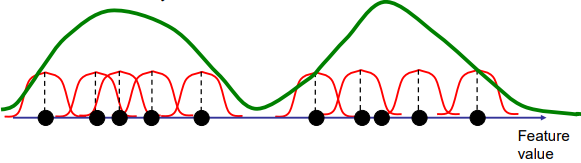
\includegraphics[height=3cm]{img/mean_shift/black_points_pdf.PNG}
    \caption{The sum of individual kernel functions functions $K(\bx - \bx_i)$.}
    %\label{fig:my_label}
\end{figure}
$f(\bx)$ approximates the probability that feature $\bx$ is observed given the data points. The maxima of $f$ (the ``modes'' of the pdf) correspond to the clusters in the data. As shown in Fig. \ref{fig:discr_points_to_cont_line}, a way to reach the peak of the PDF $f$ is by incrementing the mean by $\nabla f(\bx)$. A very rough algorithm for Mean Shift would therefore be.

\begin{algorithm}[H]
\caption{Mean shift on a very high level}
\label{alg:first_draft_mean_shift}
\begin{algorithmic}[1]
\Procedure{MeanShiftIdea} {$\bx_1,\, \bx_2, \, \ldots, \, \bx_N$} 
\For{$i=1,\ldots,N$}
\State $\bx \leftarrow \bx_i$
\While{no convergence} \Comment{gradient ascent for each point individually}
\State $\bx \leftarrow \bx_i + \nabla f(\bx) = \bx_i + \frac{1}{C}\sum \limits_{i}{\nabla K(\bx - \bx_i)}$
\EndWhile
\EndFor
\State \textbf{return} $\bx$
\EndProcedure
\end{algorithmic}
\end{algorithm}



\subsubsection{Mean Shift terminology and notation}

Before the maths is presented, this is notation that will be used.
\begin{itemize}
    \item $d$ -- the dimension of the input column vector, the entries of this vector are also called ``features''.
    \item $\bx_i$ -- the data points.
    \item ``Kernel'' $K(\bx)$ -- the function that assigns weight to every point of interest. For example, it can be Gaussian, flat, etc.
    \item ``Bandwidth'' $h$ -- the radius of the region of interest (ROI).
    \item ``PDF'' f(\bx) -- probability density function.
\end{itemize}


\subsubsection{Mathematical analysis}

A basic requirement for the kernel function, as stated in Def. \ref{def:kernel_func} is radial symmetry, i.e.
\begin{equation}
    K(\bx) = c_d k(\norm{x}^2)
\end{equation}
, where $c_d$ acts as the normalisation constant and is the volume of the $d$-dimensional sphere, such that $K(\bx)$ integrates to $1$. Some functions that can serve as the basis $k$ for the kernel are
\begin{equation}
        \textup{Epanechnikov}\quad k_E(\bx) = \left\{
\begin{array}{ll}
      1-\norm{x}^2 & \norm{x} \leq 1 \\
      0 & \textrm{otherwise}\\
\end{array} 
\right. 
    \label{eq:ep_kernel}
    \end{equation}
    \begin{equation}
        \textup{Uniform} \quad k_U(\bx) = \left\{
\begin{array}{ll}
      1 & \norm{x} \leq 1 \\
      0 & \textrm{otherwise}\\
\end{array} 
\right. 
    \end{equation}
    \begin{equation}
        \textup{Gaussian} \quad k_N(\bx) = \exp(-\frac{1}{2}\norm{x}^2)
    \end{equation}
It can be proven that the pdf function that approximates kernel density given inputs $\bx_i,\ldots, \bx_n$, where $\bx_i \in \setR^d$ is
\begin{equation}
    \hat{f}(\bx) = \frac{1}{nh^d}\sum \limits_{i=1}^{n}{K\left(\frac{\bx -\bx_i}{h} \right)}
\end{equation}
Assuming that the kernel $K(\bx)$ is differentiable, the gradient of the kernel density is
\begin{equation}
    \hat{\nabla}f(\bx) := \nabla \hat{f}(\bx) = \frac{1}{h^d}\sum\limits_{i=1}^{n}{\nabla K\left(\frac{\bx -\bx_i}{h} \right)}
\end{equation}
% ref http://cmp.felk.cvut.cz/cmp/courses/33DZOzima2007/slidy/meanShiftSeg.pdf
Computing the gradient, the derivative is
\begin{align}
    \nabla \hat{f}(\bx) &= \frac{2c_d}{nh^{d+2}} \sum \limits_{i=1} ^{n}{(\bx - \bx_i) k^{\prime}\left(\norm{\frac{\bx - \bx_i}{h}}^2\right)} \\
    &= \frac{2c_d}{nh^{d+2}}\left(\sum \limits_{i=1}^{n}{g_i} \right) 
    \underbrace{\left( \frac{\sum\limits_{i=1}^{n}{\bx_i g_i}}{\sum\limits_{i=1}^{n}{g_i}} - \bx\right)}_{\textup{mean shift vector}} ,\\
    g(r) &= k^{\prime}(r), \quad r := \norm{\bx}, \quad g_i = g(\norm{(\bx -\bx_i)/h}^2)
    \label{eq:mean_shift_vector}
\end{align}

% FIX IT!!!! http://cmp.felk.cvut.cz/cmp/courses/33DZOzima2007/slidy/meanShiftSeg.pdf and http://service.hidebux.com/index.php?q=n9XX1Z9gZ9SmlaaokJqY18qf0qdj0dWdZNygXsbUp9qcz9eU2qGk0ZiXqmOVZmSTlGOWZqjHymlj1ZSX, http://homepages.inf.ed.ac.uk/rbf/CVonline/LOCAL_COPIES/TUZEL1/MeanShift.pdf
\begin{definition} [mean shift vector]
Referring to \eqref{eq:mean_shift_vector}, 
$\sum \limits_{i=1}^{n}{g_i}$ is yet another kernel estimation and the second term $M(\bx)  = \sum\limits_{i=1}^{n}{\bx_i g_i} / \sum\limits_{i=1}^{n}{g_i} - \bx $ is the \emphasis{mean shift vector}.
\end{definition}
% ref http://homepages.inf.ed.ac.uk/rbf/CVonline/LOCAL_COPIES/TUZEL1/MeanShift.pdf
It always points toward the direction of the maximum increase in the density therefore we want to shift the current estimation $\bx$ by it in each iteration. The mean shift vector must be $\textbf{0}$ at optimum, i.e. the algorirthm stops at $\bx = \frac{\sum\limits_{i=1}^{n}{\bx_i g_i}}{\sum\limits_{i=1}^{n}{g_i}}$. This is equivalent to draft Alg. \ref{alg:first_draft_mean_shift} converging. Given this knowledge about the gradient, the latter algorithm is rewritten as follows.
% ref http://robot-develop.org/wp-content/uploads/2012/03/seg3.pdf, http://cmp.felk.cvut.cz/cmp/courses/33DZOzima2007/slidy/meanShiftSeg.pdf
\begin{algorithm}[H]
\caption{Mean shift algorithm}
\label{alg:mean_shift}
\begin{algorithmic}[1]
\Procedure{MeanShift} {$\bx_1,\, \bx_2, \, \ldots, \, \bx_n$} 
\For{$i=1,\ldots,n$}
\State $\bx \leftarrow \bx_i$
\While{no convergence} \Comment{gradient ascent for each point individually}
\State $\bx \leftarrow \bx + M(\bx) = 
 \frac{\sum \limits_{i=1}^{n}{\bx_i g\left(\norm{\frac{\bx - bx_i}{h}}^2 \right)}}%/
{\sum\limits_{i=1}^{n}{g\left(\norm{\frac{\bx - \bx_i}{h}}^2 \right)}},\quad g(\norm{\bx}) = k^{\prime}(\norm{\bx})$
\EndWhile
\EndFor
\State \textbf{return} $\bx$
\EndProcedure
\end{algorithmic}
\end{algorithm}
 \textit{guaranteed to converge}.
% ref http://robot-develop.org/wp-content/uploads/2012/03/seg3.pdf
The update step is not as complicated as it seems. For example for the kernel
\[
k(\norm{\bx}) = \left\{
\begin{array}{ll}
      1-\norm{x} & \norm{x} \leq 1 \\
      0 & \textrm{otherwise}\\
\end{array} 
\right. 
\]
, its derivative w.r.t. the distance $\norm{\bx}$ is
\[
g(\norm{\bx}) = \left\{
\begin{array}{ll}
      -1 & \norm{x} \leq 1 \\
      0 & \textrm{otherwise}\\
\end{array} 
\right. 
\]
Comparing the argument of $g$ with $1$ gives us the data points of interest therefore the ``mean'' part of $M(\bx)$ is:
\begin{align}
 \frac{\sum \limits_{i=1}^{n}{\bx_i g\left(\norm{\frac{\bx - bx_i}{h}}^2 \right)}}%/
{\sum\limits_{i=1}^{n}{g\left(\norm{\frac{\bx - \bx_i}{h}}^2 \right)}}= \frac{-\sum\limits_{\norm{\bx - \bx_i} < h}{\bx_i}} {-\sum\limits_{\norm{\bx - \bx_i} < h}1}=
\frac{\sum\limits_{\norm{\bx - \bx_i} < h}{\bx_i}}{n_h}
\label{eq:mean_shift_mean_upd}
\end{align}
$n_h$ is simply the number of inside the kernel, for which $\norm{\bx - \bx_i} < h$ and $\sum\limits_{\norm{\bx - \bx_i} < h}{\bx_i}$ is just the average of the data points within a radius $h$ of $\bx$! Regarding the convergence of the algorithm the following can be proved.
\begin{theorem}
If the kernel function $k(\bx)$ is convex and monotonically decreasing then the update of $\bx$ converges and the pdf $\hat{f}(\bx)$ increases.
\end{theorem}
For the Epanechnikov kernel, convergence is reached in finite number of steps. Finally, mean shift runs in $\mathcal{O}(n^2T)$, where $n$ is the number of input points and $T$ the number of iterations.








% cont here http://campar.in.tum.de/pub/benz2014clust/benz2014clust.poster.pdf, http://campar.in.tum.de/twiki/pub/Chair/TeachingWs12TDCV/mean_shift.pdf , https://bzdww.com/article/168933/, http://cmp.felk.cvut.cz/cmp/courses/33DZOzima2007/slidy/meanShiftSeg.pdf, http://homepages.inf.ed.ac.uk/rbf/CVonline/LOCAL_COPIES/TUZEL1/MeanShift.pdf, https://books.google.de/books?id=bXzAlkODwa8C&pg=PA258&lpg=PA258&dq=mean+shift++kernel+function+derivative&source=bl&ots=g_064_jEzE&sig=ACfU3U1enuWtaZzqKxcZ-L-T21T8EcasKQ&hl=en&sa=X&ved=2ahUKEwixv8Sd9q7hAhWFJlAKHXraBAM4ChDoATAJegQICRAB#v=onepage&q=mean%20shift%20%20kernel%20function%20derivative&f=false
% conv proof: https://pdfs.semanticscholar.org/3753/29683956d3cea5b501d161766bc84a4fd608.pdf


\subsubsection{Mean Shift as a tool for segmentation}

When we want to segment an image, it is usually converted from RGB to another colour space such as HSV or LUV. In this case, suppose the image is in LUV.

Then the feature space is $(l, u, v, x, y)$. To perform segmentation, we apply \textit{two different} mean shifts in the 5-dimensional space as we want to segment pixels based on their location and colour. For each pixel $(x_i,y_i)$ of intensity color $(l_i, u_i, v_i)$, find the corresponding mode $c_{col}$. All of the pixels $(x_i,y_i)$  corresponding to the same
mode $c_{col}$ are grouped into a single region. At the same time, mean shift is performed in the 2D space $xy$ and all of the corresponding pixels $(x_i,y_i)$ are grouped into a single mode $c_{pos}$. The kernel in this case is the product of the position kernel and the colour kernel,
\begin{equation}
    K_{pos,col}(\bx) = \frac{c}{h_{col}^3 h_{pos}^2}\,
    k\left(\frac{\norm{\bx_{pos}}^2}{h_{pos}^2} \right)
    k\left(\frac{\norm{\bx_{col}}^2}{h_{col}^2} \right)
\end{equation}
\begin{figure}[H]
    \centering
    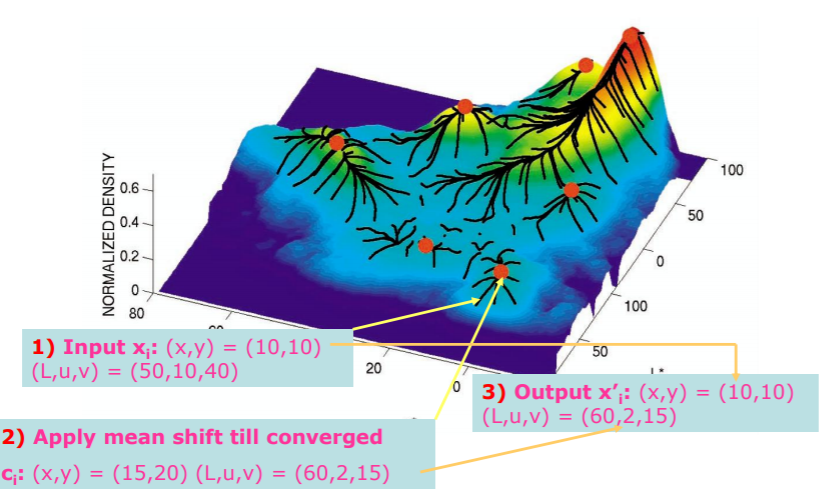
\includegraphics[height=4.5cm]{img/mean_shift/mean_shift_5d.PNG}
    \caption{Mean shift in the LUV space.}
\end{figure}

\subsubsection{Mean Shift as a tracker}


The idea behind using it as a tracker is the following. Given a frame that contains the object of interest (OOI), we want to successfively move the window of radius $h$ towards the ``centre'' of the object. How is the centre defined?

% ref https://docs.opencv.org/3.4.1/db/df8/tutorial_py_meanshift.html
After selecting a sample of the OOI, backprojection from the previous section helps create a greyscale. salience (likelikehood) frame (see $b$ matrix in backprojection section). In this frame, the whiter the pixel, the more likely it is to belong to the OOI.

Then, mean shift can be performed in 3D - $(x,y,i)$, where $i$ is the salience intensity to chase the object and output its $(x,y)$.


\subsubsection{Implementation from scratch}

Below are the main features of my own adaptation of mean shift.
\begin{itemize}
    \item Mean shift is performed in the $xy$ space so the ``mode'' (converge) centre is 2D.
    \item If it performed in $xy$ space, which points are considered? The candidate points are the result of backprojecting a sample of the OOI to the frame, create a likelihood frame $b$, as described in Section 1.1. Then they are automatically thesholded, which yields a BW frame. For that frame, the white points are likely to belong to the OOI and the black are irrelevant. So we want to generate a pdf from those white points and find its centre of density.
    \item The chosen mean shift kernel if $k(r) = 1 - r, \; r \leq 1, \; r = \norm{x}$. The radius of interest can be chosen by the user but defaulted to some small value anyway. Therefore the update step of the m.s. vector $x$ is simple -- it is simply the centroid of all points up to distance $h$ around $x$ as derived in \ref{eq:mean_shift_mean_upd}.
\end{itemize}
My implementation code is listed in \ref{app:hist_backproj_src}. The program is standalone and expect a video path and a radius from the user. Below are some representative outputs for a football sequence. For that particular scane, the player was successfully tracked for the majority of the frames.

\begin{multicols}{3}
\begin{figure}[H]
    \centering
    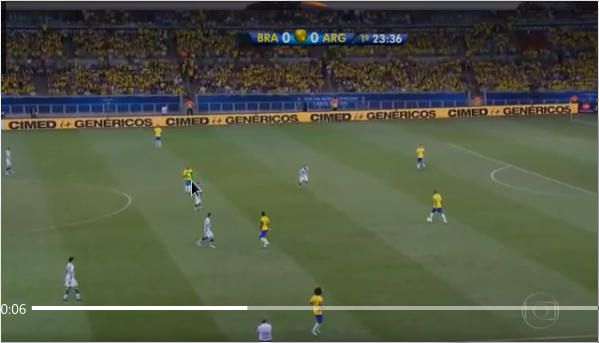
\includegraphics[width=.33\textwidth]{img/mean_shift/out_my_ms1.png}
    \caption{Initial step; grabbing a sample of the player to track (green box).}
    %\label{fig:my_label}
\end{figure}
\columnbreak
\begin{figure}[H]
    \centering
    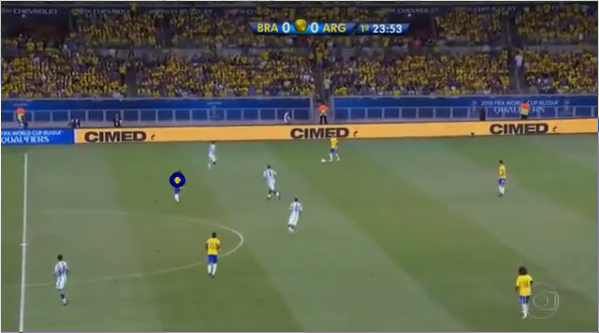
\includegraphics[width=.33\textwidth]{img/mean_shift/out_my_ms2.png}
    \caption{An intermediate tracking step (blue circle).}
    %\label{fig:my_label}
\end{figure}
\columnbreak
\begin{figure}[H]
    \centering
    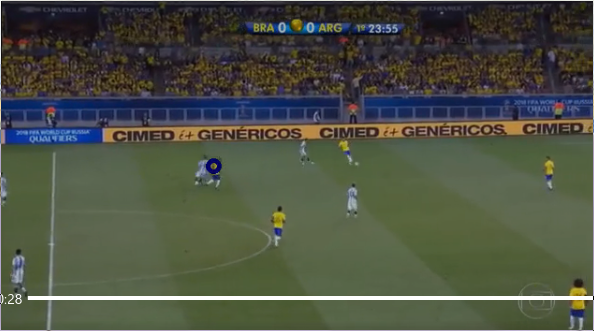
\includegraphics[width=.33\textwidth]{img/mean_shift/out_my_ms3.png}
    \caption{Player keeps being tracked right after being blocked by another player.}
    %\label{fig:my_label}
\end{figure}
\columnbreak
\end{multicols}


The algorithm is robust given that the sample represents reasonably well the OOI. It is not robust when the scale of the OOI changes, e.g. in car scenes when a car to be tracked car is initially in the background and in the end approaches the camera. Then mean shift variations that are able to adapt the radius $h$ need to be considered and there's a good amount of literature on that.


\subsubsection{Implementation in OpenCV}

% ref https://docs.opencv.org/3.3.0/db/df8/tutorial_py_meanshift.html
Mean shift in OpenCV consists of the following main stages:
\begin{enumerate}
    \item Set up a target; i.e. grab a sample of the OOI. Once again, the OOI shouldn't be in RGB, but in a colour space that decouples hue and illumiation.
    \item Provide an initial window -- essentially initialise the mean shift tracking vector $x$ and provide a radius $h$ to define the area around $\bx$ where points for the update of $\bx$ will be considered.
    \item Perform backprojection of the target on the current frame, generating a greyscale image. Perform mean shift on the greyscale backprojected image. 
\end{enumerate}
After grabbing the ROI (in HSV), the OpenCV approach also filters only certain H (0 to 180 -- maximum is 180), S (60 to 255 -- maximum is 255), V (32 to 255 -- maximum is 255) bands in order to remove potential noise:
\begin{minted}{python}
mask = cv2.inRange(hsv_roi, np.array((0., 60.,32.)), np.array((180.,255.,255.)))
\end{minted}
Mean shift is performed, for instance, as:
\begin{minted}{python}
cv2.meanShift(probImage, track_window, criteria) -> retval, track_window
\end{minted}
\begin{itemize}
    \item \mintinline{python}{probImage}: greyscale backprojected frame.
    \item \mintinline{python}{track_window}: the updated tracking window as \mintinline{python}{x, y, w, h} (essentially the updated m.s. vector).
    \item \mintinline{python}{term_crit}: termination criteria, e.g. to set them to 10 iterations or window displacement no more than 1 pixel do \mintinline{python}{( cv2.TERM_CRITERIA_EPS | cv2.TERM_CRITERIA_COUNT, 10, 1)}.
    \item \mintinline{python}{retval}: A boolean whether the algorithm was successful.
    \item \mintinline{python}{track_window}: The updated tracking window in the same format as the old one.
\end{itemize}
The code provided by OpenCV's documentation has been lazily re-written and made interactive as listed in \ref{app:mean_shift_opencv}. The user can define the bounding box around the object of interest and then press \mintinline{python}{q} to finalise the selection and start the algorithm.




\subsubsection{Mean Shift pros and cons}
% ref http://www.cs.ucf.edu/~bagci/teaching/computervision16/Lec11.pdf
\begin{multicols}{2}
    \begin{itemize}
        \item[\textcolor{DarkPink}{\ding{51}}] Does not assume spherical clusters.
        \item[\textcolor{DarkPink}{\ding{51}}] Just a single parameter (window size).
        \item[\textcolor{DarkPink}{\ding{51}}]
        Finds variable number of modes.
        \item[\textcolor{DarkPink}{\ding{51}}]
        Robust to outliers.
    \end{itemize}
    
    \columnbreak
    \begin{itemize}
        \item[\textcolor{DarkPink}{\ding{55}}] 
        Output depends on window size.
        \item[\textcolor{DarkPink}{\ding{55}}]
        Computationally expensive (however, not impossible to use in real time).
        \item[\textcolor{DarkPink}{\ding{55}}]
        Does not scale well with dimension of feature space.
    \end{itemize}
\end{multicols}




\subsection{Camshift (Continuously Adaptive Mean Shift)}





%------------------------------ New section ------------------------------%

\section{Motion-based methods}

\subsection{Optical Flow}



\subsection{Lukas-Kanade tracking}





%%%%%%%%%%%%%%%%%%%%%%%%%%%%%%%%%%%%%%%%%%%%%%%%%%%%%%%%%%%%%%%%%%%%%%%%%%%%%%%%%%%%%%%%%%%%%%%%%%%%
% APPENDICES
%%%%%%%%%%%%%%%%%%%%%%%%%%%%%%%%%%%%%%%%%%%%%%%%%%%%%%%%%%%%%%%%%%%%%%%%%%%%%%%%%%%%%%%%%%%%%%%%%%%%
\newpage
\appendix

\section{Appendices}

% ------------------------ New appendix ------------------------ %
\newpage
\subsection{HSV domain}
\label{app:hsv_domain}






% ------------------------ New appendix ------------------------ %
\newpage


\subsection{Histogram backprojection implementation from scratch -- source code}
\label{app:hist_backproj_src}
\lstinputlisting[language=python,caption={Histogram backprjection from scratch (\detokenize{src/hist_backproj/backproj.py)}.}, label=src:mylabel]{src/hist_backproj/backproj.py}



% ------------------------ New appendix ------------------------ %
\newpage
\subsection{Histogram backprojection implementation using OpenCV - source code}
\label{app:hist_backproj_src_opencv}
\lstinputlisting[language=python,caption={Histogram backprjection using OpenCV's \mintinline{python}{calcBackProject} (\detokenize{src/hist_backproj/backproj_cv.py)}.}]{src/hist_backproj/backproj_cv.py}
%\inputminted{python}{src/hist_backproj/backproj_cv.py}


% ------------------------ New appendix ------------------------ %
\newpage
\subsection{My mean shift implementation from scratch -- source code}
\label{app:mean_shift_mine}
\lstinputlisting[language=python,caption={Mean shift using OpenCV's \mintinline{python}{meanShift} (\detokenize{src/mean_shift/my_mean_shift.py)}.}]{src/mean_shift/my_mean_shift.py}
%\inputminted{python}{src/hist_backproj/backproj_cv.py}


% ------------------------ New appendix ------------------------ %
\newpage
\subsection{Mean Shift implementation using OpenCV - source code}
\label{app:mean_shift_opencv}
\lstinputlisting[language=python,caption={Mean shift using OpenCV's \mintinline{python}{meanShift} (\detokenize{src/mean_shift/mean_shift_cv.py)}.}]{src/mean_shift/mean_shift_cv.py}
%\inputminted{python}{src/hist_backproj/backproj_cv.py}

\end{document}